\documentclass{beamer}
\usepackage[ngerman]{babel}
\usepackage[utf8]{inputenc}
\usepackage{mdframed}

\newmdtheoremenv{theo}{Definition}
\newcommand\blfootnote[1]{%
	\begingroup
	\renewcommand\thefootnote{}\footnote{#1}%
	\addtocounter{footnote}{-1}%
	\endgroup
}

\title{Argument Search}
\subtitle{Einleitung und aktueller Stand}
\author{Florian Euchner \and Nick Heilenkötter \and Nico Weidmann}
\date{20. August 2018}

\begin{document}
	\begin{frame}
		\maketitle
	\end{frame}

	\begin{frame}{Gliederung}
		\tableofcontents
	\end{frame}

	\section{Problemstellung}
	\begin{frame}{Problemstellung}{Warum Argumentsuche?}
		\begin{itemize}[<+->]
			\item Meinungsbildung
			\begin{itemize}
				\item gelesene/gehörte Meinung überprüfen
			\end{itemize}
			\item Argumentationshilfe
			\begin{itemize}
				\item moralische Fragestellungen oder aktuelle Themen
			\end{itemize}
			\item Gegenargumente zur eigenen Sicht
			\begin{itemize}
				\item Position des politischen Gegners verstehen
			\end{itemize}
		\item[] \textbf{Ziel:} reflektierte Sicht auf gesellschaftliche Fragestellungen
		\end{itemize}
	\end{frame}

	\begin{frame}{Problemstellung}{Warum nicht Google?}
		\begin{itemize}[<+->]
			\item Suchbegriff nimmt Antwort vorweg: Keine neutrale, umfassende Information
			\alt <1, 2>{
				\begin{figure}
					\includegraphics<1>[width=0.8\textwidth]{img/s21_pro.png}
					\includegraphics<2>[width=0.8\textwidth]{img/s21_contra.png}
					\caption{Google-Suche nach S21 mit positiv / negativ konnotierten Begriffen}
				\end{figure}
			}{}
			\item<3-> Ergebnisse nach Relevanz, nicht Qualität sortiert
			\item<4-> Keine Trennung von Thesen und Argumenten
			\item<5-> Schwer verständlich: Lange Artikel, viel Text
			\item<6-> Erkennung von Trugschlüssen, Verschwörungstheorien bleibt Nutzer überlassen
			\item<7-> Suchmaschinen nehmen gesellschaftliche Verantwortung kaum wahr
		\end{itemize}
	\end{frame}

	\section{Argumentationstheorie}
	\begin{frame}{Argumente}{Wonach suchen wir eigentlich?}
		\begin{quote}
			"[An argument is] a collection of truth-bearers (that is, the things that bear truth and falsity, or are true and false) some of which are offered as reasons for one of them, the conclusion."
			\flushright \tiny Matthew McKeon in: Internet Encyclopedia of Philosophy, Eintrag ''Argument''
		\end{quote}
		\begin{itemize}[<+->]
			\item Prämissen $\Rightarrow$ Konklusion
			\item was ist ein gutes und was ein schlechtes Argument?
		\end{itemize}
	\end{frame}
	\begin{frame}{Klassifizierung von Argumenten}{Argumentationstheorie}
		logisch ("Fehlerhaftigkeit"):
		\begin{itemize}[<+->]
			\item Gültigkeit
			\begin{itemize}
				\item aus den Prämissen lässt sich logisch die Konklusion folgern
			\end{itemize}
			\item Schlüssigkeit
			\begin{itemize}
				\item gültig und die Prämissen sind wahr
			\end{itemize}
		\end{itemize}
		subjektiv ("Überzeugungskraft")		\begin{itemize}[<+->]
			\item Konkretheit
			\item Ausrichtung auf den Adressaten
			\item Formulierung - moralisch/emotional/plausibel
		\end{itemize}
	\end{frame}
	\begin{frame}{Klassifizierung von Argumenten}{Eine Taxonomie der Argumentationsqualität}
		\begin{figure}
			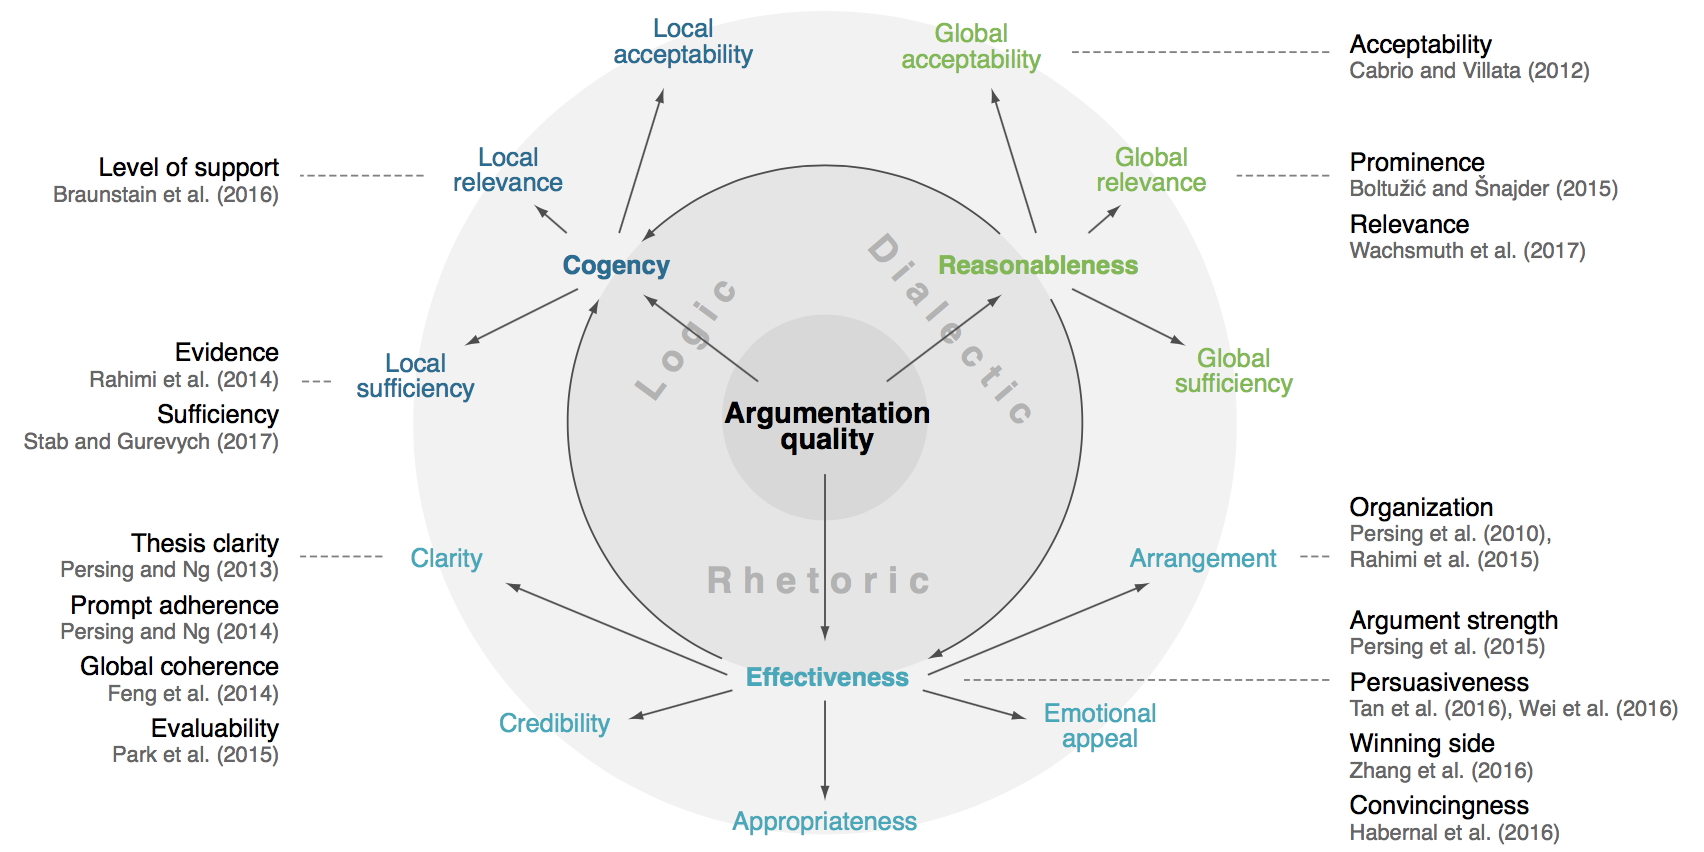
\includegraphics[width=\textwidth]{img/discussion-taxonomy}
			\caption{\small Wachsmuth, Henning, et al. ``Computational argumentation quality assessment in natural language.'' \textit{Proceedings of the 15th Conference of the European Chapter of the Association for Computational Linguistics: Volume 1, Long Papers}. Vol. 1. 2017.}
		\end{figure}
	\end{frame}

		\begin{frame}{Klassifizierung von Argumenten}{Schlechte Argumente - Trugschlüsse (\textit{fallacies})}
		\begin{itemize}[<+->]
			\item Persönlicher Angriff (\textit{ad hominem})
			\begin{quote}
				\small You are the single biggest liar, you probably are worse than Jeb Bush.
				\begin{flushright}
					\tiny Donald Trump zu Ted Cruz
				\end{flushright}
			\end{quote}
			\item Strohmann (\textit{straw man})
			\begin{quote}{}
				\small Over and over, we have been told by our opponents that bigger tax cuts and fewer regulations are the only way.
				\begin{flushright}
					\tiny Barack Obama vor der DNC, 2012
				\end{flushright}
			\end{quote}
			\item Falsches Dilemma (\textit{false dichotomy})
			\begin{quote}{}
				\small Every nation, in every region, now has a decision to make. Either you are with us, or you are with the terrorists.
				\begin{flushright}
					\tiny George W. Bush nach 9/11
				\end{flushright}
			\end{quote}
			\item uvm. \footnote{Siehe auch \href{https://en.wikipedia.org/wiki/List_of_fallacies}{Wikipedia: List of fallacies}}
		\end{itemize}
	\end{frame}

	\begin{frame}{Probleme bei der Argumentensuche}{Psychologie - Kognitive Verzerrungen (\textit{cognitive biases})}
		\begin{itemize}
			\item Bestätigungsfehler (\textit{confirmation bias})
			\item Congruence bias
			\item Dunning–Kruger effect
			\item Stereotypisierung
			\item Gerechte-Welt-Glaube (\textit{just-world hypothesis})
			\item uvm. \footnote{Siehe auch \href{https://en.wikipedia.org/wiki/List_of_cognitive_biases}{Wikipedia: List of cognitive biases}}
		\end{itemize}
	\end{frame}

	\section{Lösungsansätze}
	\subsection{Suchmaschinen und Retrievalmodelle}

	\begin{frame}{Suchmaschinen}{Suche durch Information Retrieval}
		\begin{itemize}[<+->]
			\item computergestütztes Suchen nach komplexen Inhalten (hier: Textpassagen)
			\item verschiedene Modelle zur Auswahl relevanter Ergebnisse
			\item Relevanz nicht binär: Sortierung der Ausgabe
			\item verschiedene Modelle:
			\begin{itemize}
				\item linktopologische Modelle (z.B. Google)
				\item Nutzer-Nutzungsmodell
				\item $\ldots$
				\item Textstatistik
				\begin{itemize}
					\item Divergence From Randomness (DFR)
				\end{itemize}
			\end{itemize}
		\end{itemize}
	\end{frame}

	\begin{frame}{Divergence From Randomness}
		\begin{itemize}
			\item probabilistisches gewichtetes Information Retrieval
			\item Ziel: Informationsgehalt eines Dokuments ermitteln
		\end{itemize}
		\begin{itemize}[<+->]
			\item Gewichtung \blfootnote{Siehe auch: \href{http://www.is.informatik.uni-duisburg.de/bib/pdf/ir/Abolhassani_Fuhr_04.pdf}{Abolhassani und Fuhr: Divergence From Randomness Approach for Content-Only Search in XML Documents}}
			\begin{itemize}
				\item je häufiger das Wort, desto relevanter
				\item je seltener das Wort erwartet wurde (nach zufälliger Verteilung), desto relevanter ist das Vorkommen
			\end{itemize}
			\item ''elite set'' aus den Dokumenten, in denen das Wort (häufig) vorkommt
			\item gemeinsam mit Auftreten in allen Dokumenten: Häufigkeitsverteilung aus einem zu wählenden Zufallsmodell
		\end{itemize}
	\end{frame}

	\begin{frame}{mögliche Erweiterung der Modelle}{Proximity}
		\begin{itemize}[<+->]
			\item zusätzliche Berücksichtigung der Nähe der Anfrageterme zueinander
			\item Dokumente in denen die gesuchten Terme dicht beieinander liegen sind relevanter
			\item z.B. durch Markov Random Fields (MRF) \blfootnote{Siehe auch: \href{http://terrier.org/docs/v3.5/javadoc/org/terrier/matching/dsms/MRFDependenceScoreModifier.html}{terrier.org}}
		\end{itemize}
	\end{frame}

	\subsection{Bestehende Suchmaschinen}
	\begin{frame}{Existierende Argument-Suchmaschinen}
		\begin{itemize}
			\item args (\url{args.me})
			\item ArgumenText (\url{www.argumentsearch.com})
		\end{itemize}
	\end{frame}
	\begin{frame}{args}
		\begin{itemize}
			\item Entwickelt an der Bauhaus-Universität Weimar
			\item Index bestehend aus 291.440 Argumenten
			\begin{itemize}
				\item geschürft von 5 Debattierportalen
				\item bestehende Struktur der Debatten genutzt
			\end{itemize}
			\item Annotation der Argumente mit ``Pro'' und ``Con''
			\item Implementierung basierend auf Apache UIMA und Apache Lucene
		\end{itemize}
		~\\
		\tiny Wachsmuth, Henning, et al. ``Building an argument search engine for the web.''
		\textit{Proceedings of the 4th Workshop on Argument Mining}. 2017.
	\end{frame}
	\begin{frame}{args}
		\begin{figure}
			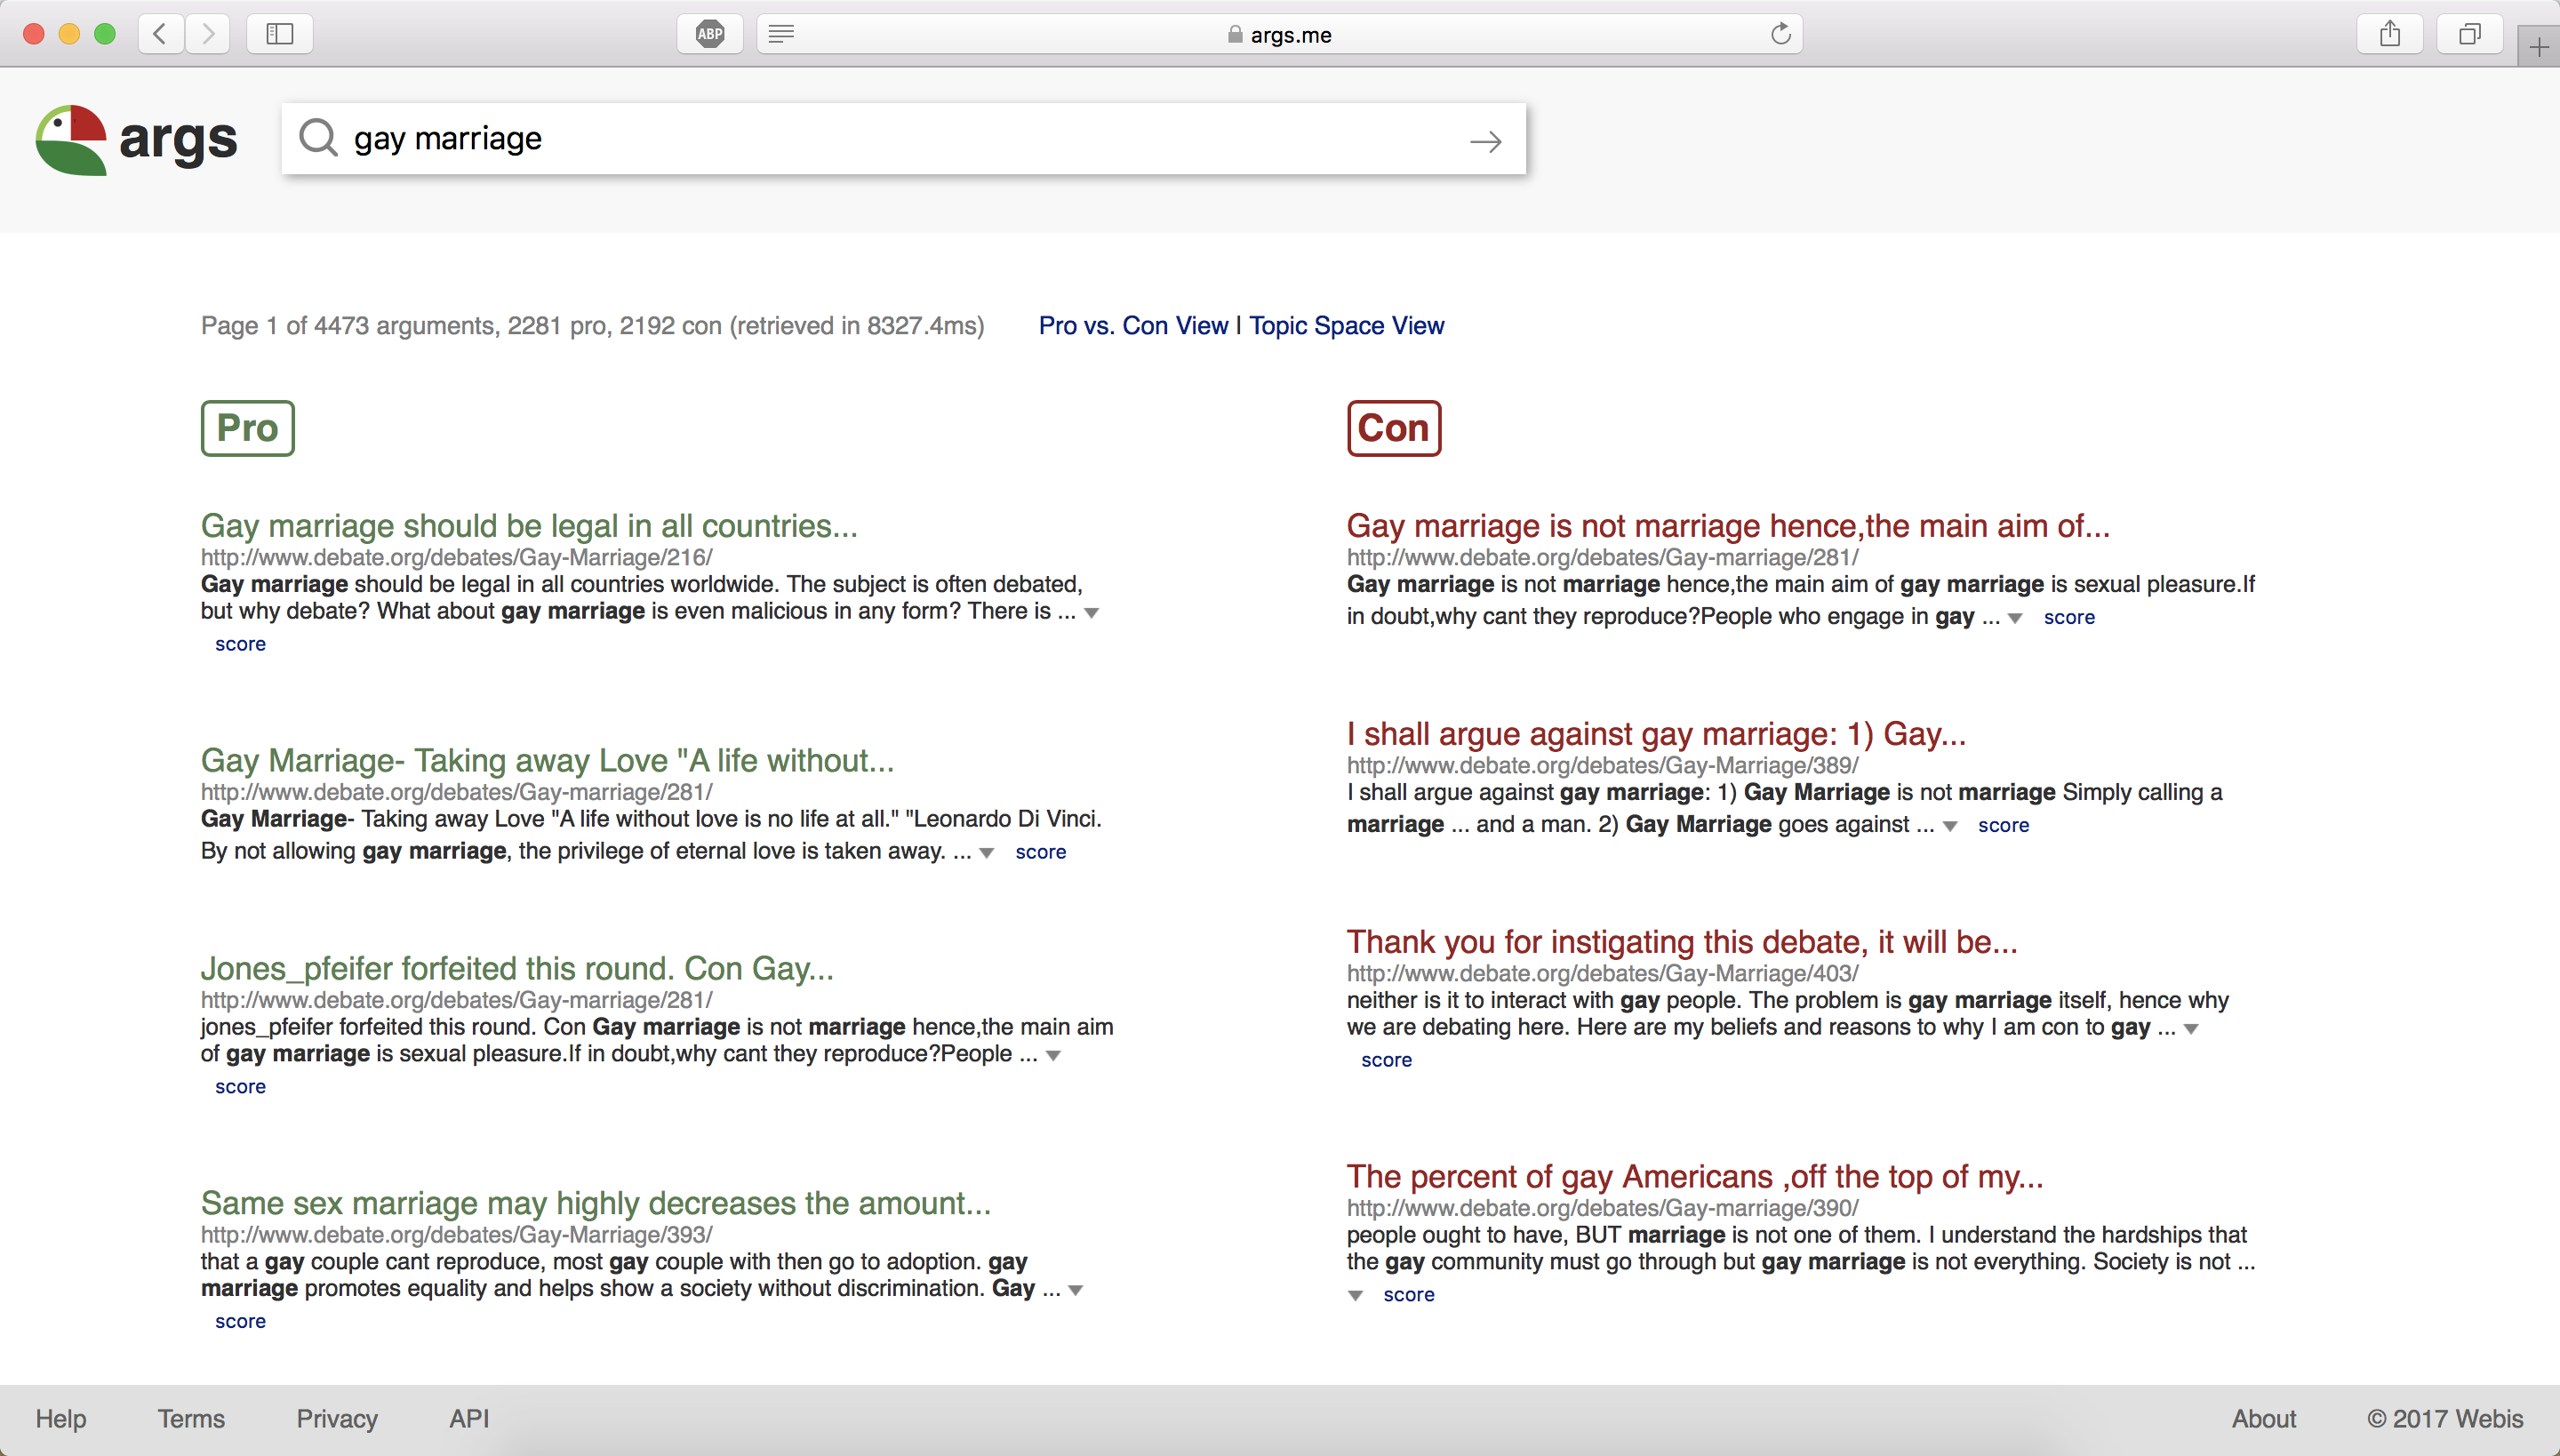
\includegraphics[width=\textwidth]{img/args-screenshot-gay-marriage}
			\caption{Suche nach ``gay marriage'' mit args, Pro/Con-Ansicht}
		\end{figure}
	\end{frame}
	\begin{frame}{ArgumenText}
		\begin{itemize}
			\item Entwickelt an der TU Darmstadt
			\item 400 Mil. heterogene englische Textdokumente
			\begin{itemize}
				\item basierend auf CommonCrawl
				\item keine Debattenstruktur / annotierte Argumente
			\end{itemize}
			\item Indexing und Retrieval basierend auf Elasticsearch
			\item Identifikation der Argumente nach Retrieval durch ein neuronales Netz
		\end{itemize}
		~\\
		\tiny Stab, Christian, et al. ``ArgumenText: Searching for Arguments in Heterogeneous Sources.''
		\textit{Proceedings of the 2018 Conference of the North American Chapter of the Association for
		Computational Linguistics: Demonstrations}. 2018.
	\end{frame}
	\begin{frame}{ArgumenText}
		\begin{figure}
			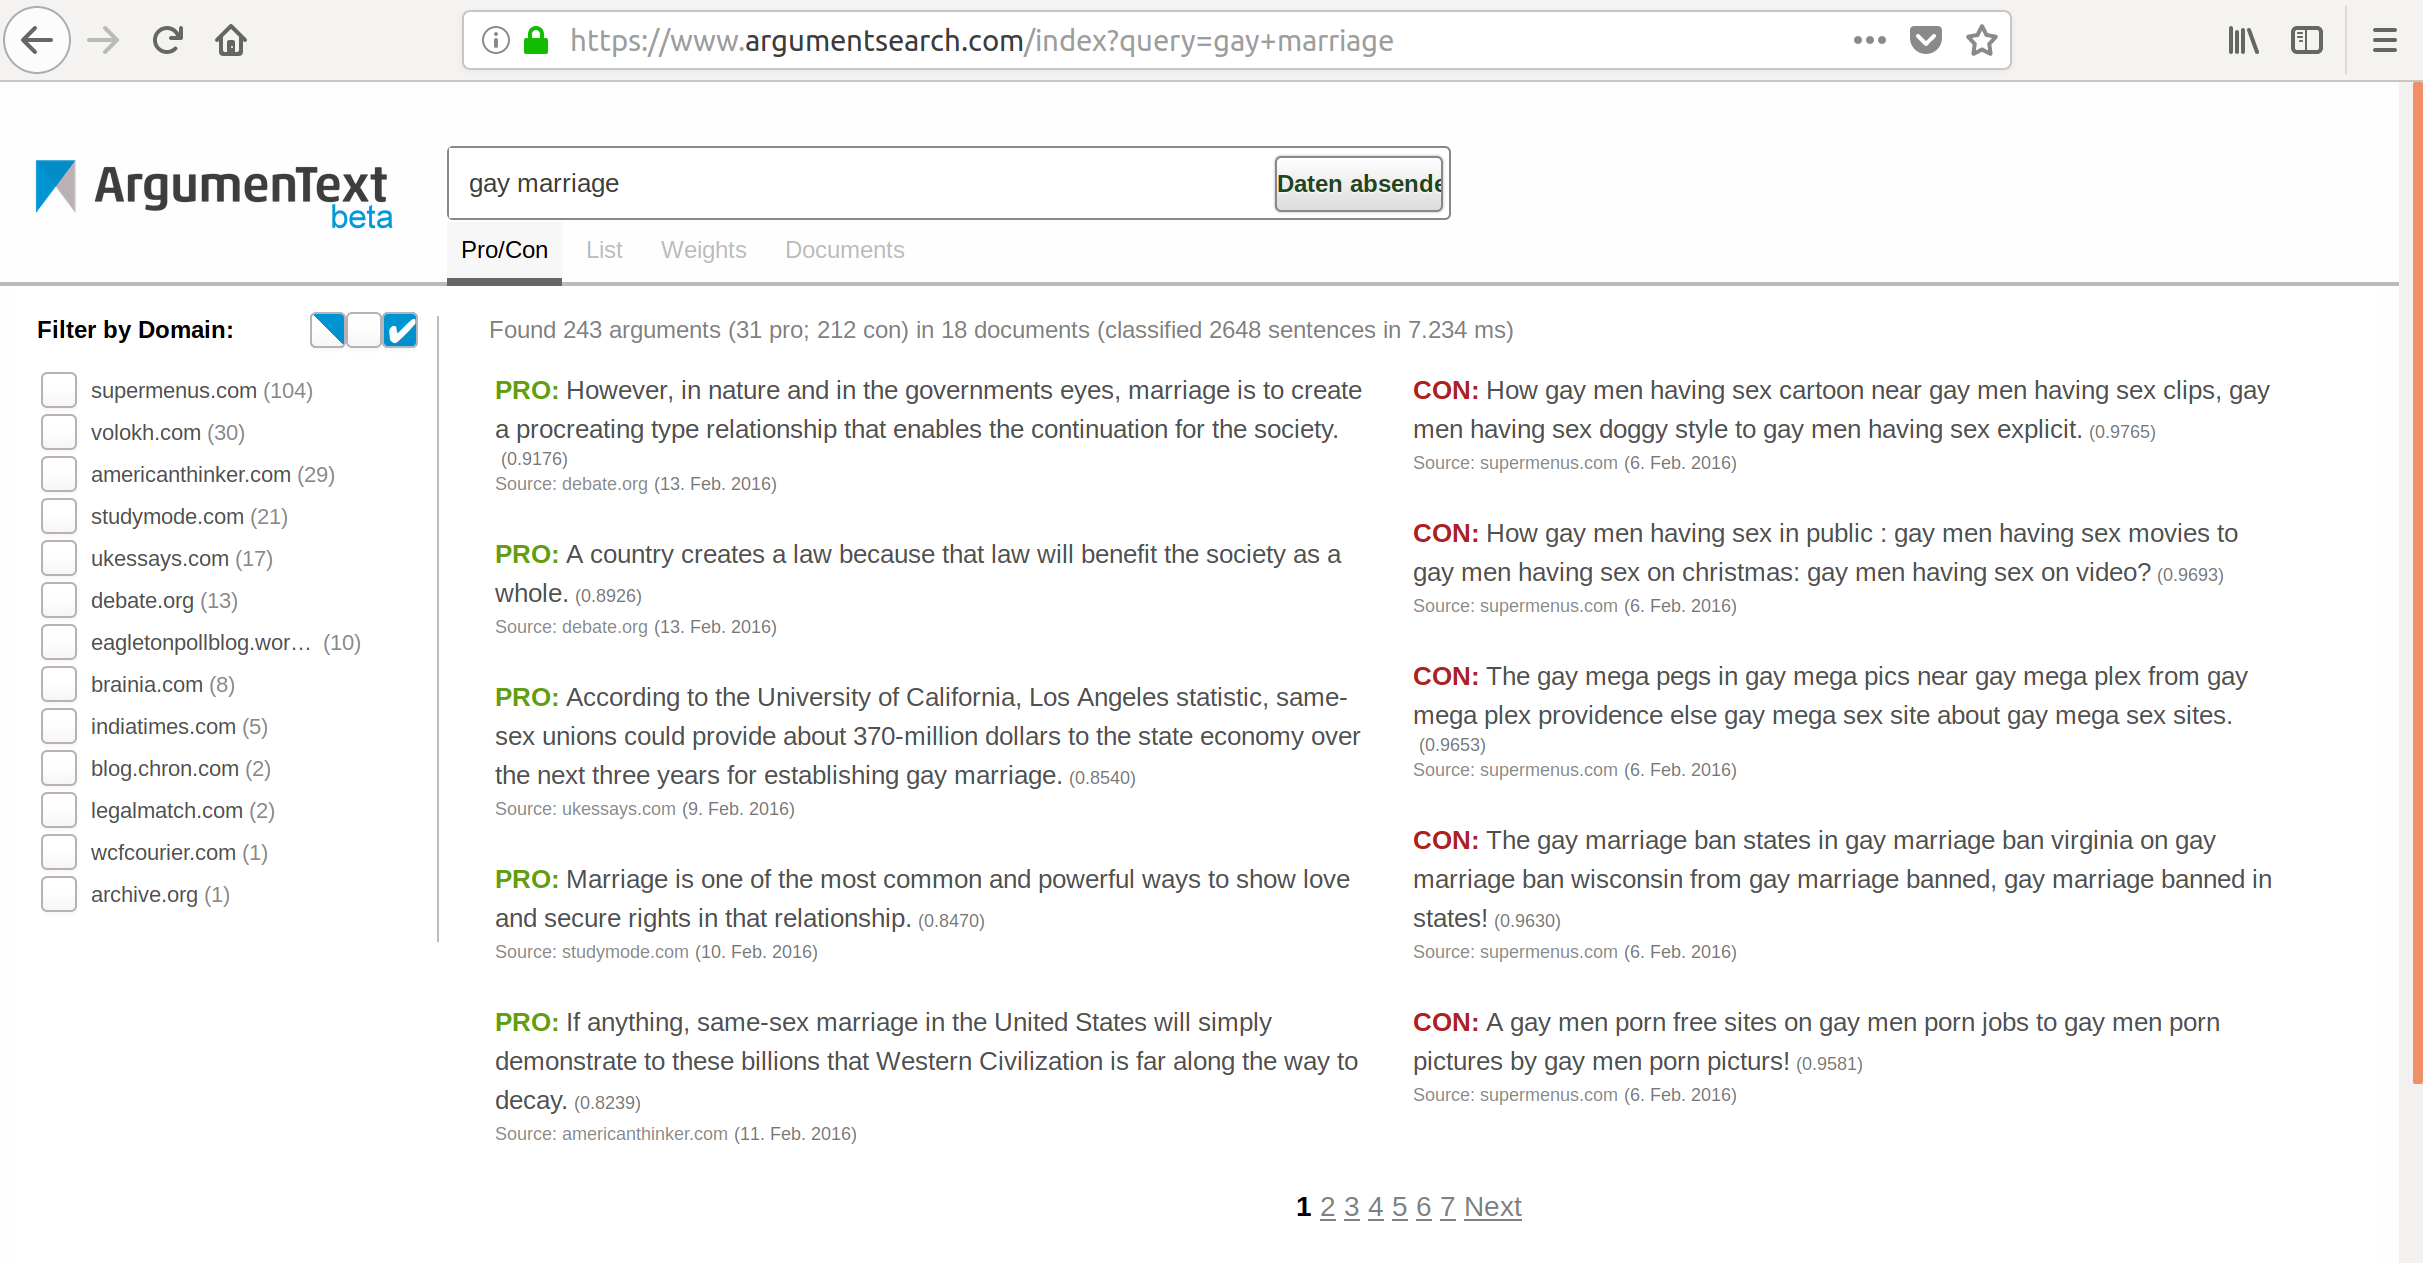
\includegraphics[width=\textwidth]{img/argumentext-screenshot-gay-marriage}
			\caption{Suche nach ``gay marriage'' mit ArgumenText}
		\end{figure}
	\end{frame}

	\subsection{Lösungsvorschlag / Arbeitshypothese}
	\begin{frame}{Lösungsvorschlag / Arbeitshypothese}{Die ideale Suchmaschine}
		\begin{block}{Informationsbeschaffung mit Argumentensuche sollte sein...}
			\begin{itemize}
				\item Zum Suchbegriff passend
				\item Neutral, verschiedene Thesen mit ``Pro'' und ``Contra''
				\item Umfassend, Argumente nach Qualität sortiert
				\item Leicht und schnell verständlich
				\item Trugschlüsse und ``kontroverse Theorien'' werden nicht versteckt, aber als solche markiert
				\item Menschliche Psychologie sollte beim Design einer Suchmaschine berücksichtigt werden
			\end{itemize}
		\end{block}
		\begin{block}{Grundproblem: Filter bubbles / Echokammern / Fake news}
			Suchmaschine soll auch bei kontroversen Themen funktionieren!
		\end{block}
	\end{frame}

	\begin{frame}{Arbeitshypothese\only<2->{n}}
		\begin{itemize}[<+->]
			\item Durch die Wahl eines geeigneten \textbf{Retrievalmodells} lässt sich die Relevanz der Suchergebnisse verbessern
			\item Unter Einbeziehung der Top-Answers auf Q\&A-Plattformen ist eine \textbf{halb-automatische Evaluierung} der Ergebnisse von Argumentsuchmaschinen möglich
		\end{itemize}
	\end{frame}

	\section{Roadmap}
	\begin{frame}{Roadmap}
		%todo: was wollen wir noch tun? Suchmaschinen vergleichen/bewerten..
		\begin{enumerate}
			\item \textbf{Implementierung einer Argument-Suchmaschine}
			\begin{itemize}
				\item Terrier IR Platform (moderne Retrievalmodelle)
				\item \url{args.me}-Datensatz
			\end{itemize}
			\item \textbf{Implementierung einer Evaluierungsplattform} zur Bewertung von Suchmaschinen
			\begin{itemize}
				\item Test anhand ausgewählter Suchanfragen
				\item Pooling der Top-Suchergebnisse von args und eigener Implementierung
				\item Bewertung der Suchergebnisse durch Assessoren
			\end{itemize}
			\item \textbf{Alternative Evaluierungsmethode}: halbautomatische Evaluierung
			\begin{itemize}
				\item Nutzung von ``best answers'' auf Q\&A-Plattformen (Yahoo-Answers, /r/ChangeMyView)
				\item Bestimmung der Ähnlichkeit der Suchergebnisse zur Argumentation in der best answer
			\end{itemize}
		\end{enumerate}
	\end{frame}
	\begin{frame}{Aktueller Stand}
		\begin{itemize}
			\item Suchmaschine auf Basis von Terrier implementiert
			\begin{itemize}
				\item \url{args.me}-Datensatz für Terrier indiziert
				\item Suche über einheitliche API möglich
			\end{itemize}
			\item Beginn der Implementierung der Evaluierungsplattform
			\item Erste Überlegungen zu halbautomatischer Evaluierung
			\begin{itemize}
				\item Posts und Kommentare von \url{/r/ChangeMyView}?
			\end{itemize}
		\end{itemize}
		\begin{figure}
			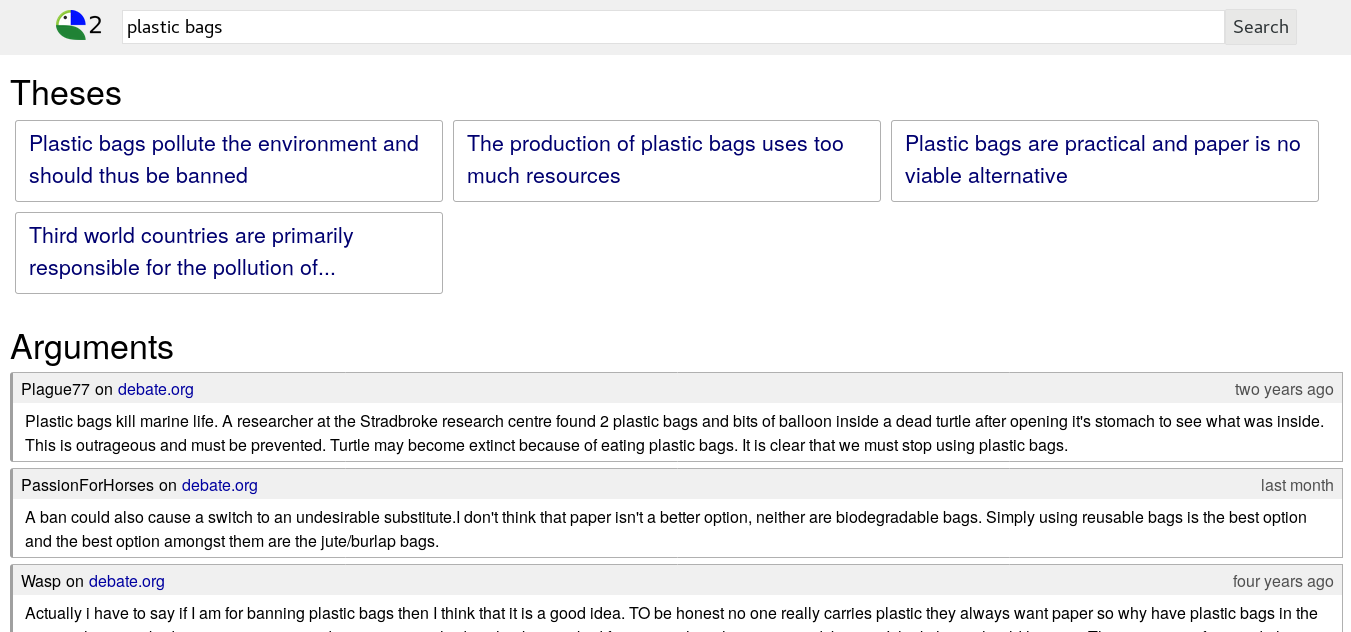
\includegraphics[width=0.95\textwidth]{img/searchui-prototype}
		\end{figure}
	\end{frame}
	\begin{frame}{Nächste Schritte}
		\begin{itemize}
			\item Bestimmung der häufigsten Themen im Datensatz
			\item Auswahl der zur Evaluierung genutzten Informationsbedürfnisse und Suchanfragen
			\item Festlegung der Qualitätskriterien zur Evaluierung\\
			$\Rightarrow$ was sind ``gute'' Argumente?
		\end{itemize}
	\end{frame}

	\begin{frame}{Relevanz von Argumenten}{Was sind ``passende'' Argumente?}
		\begin{figure}
			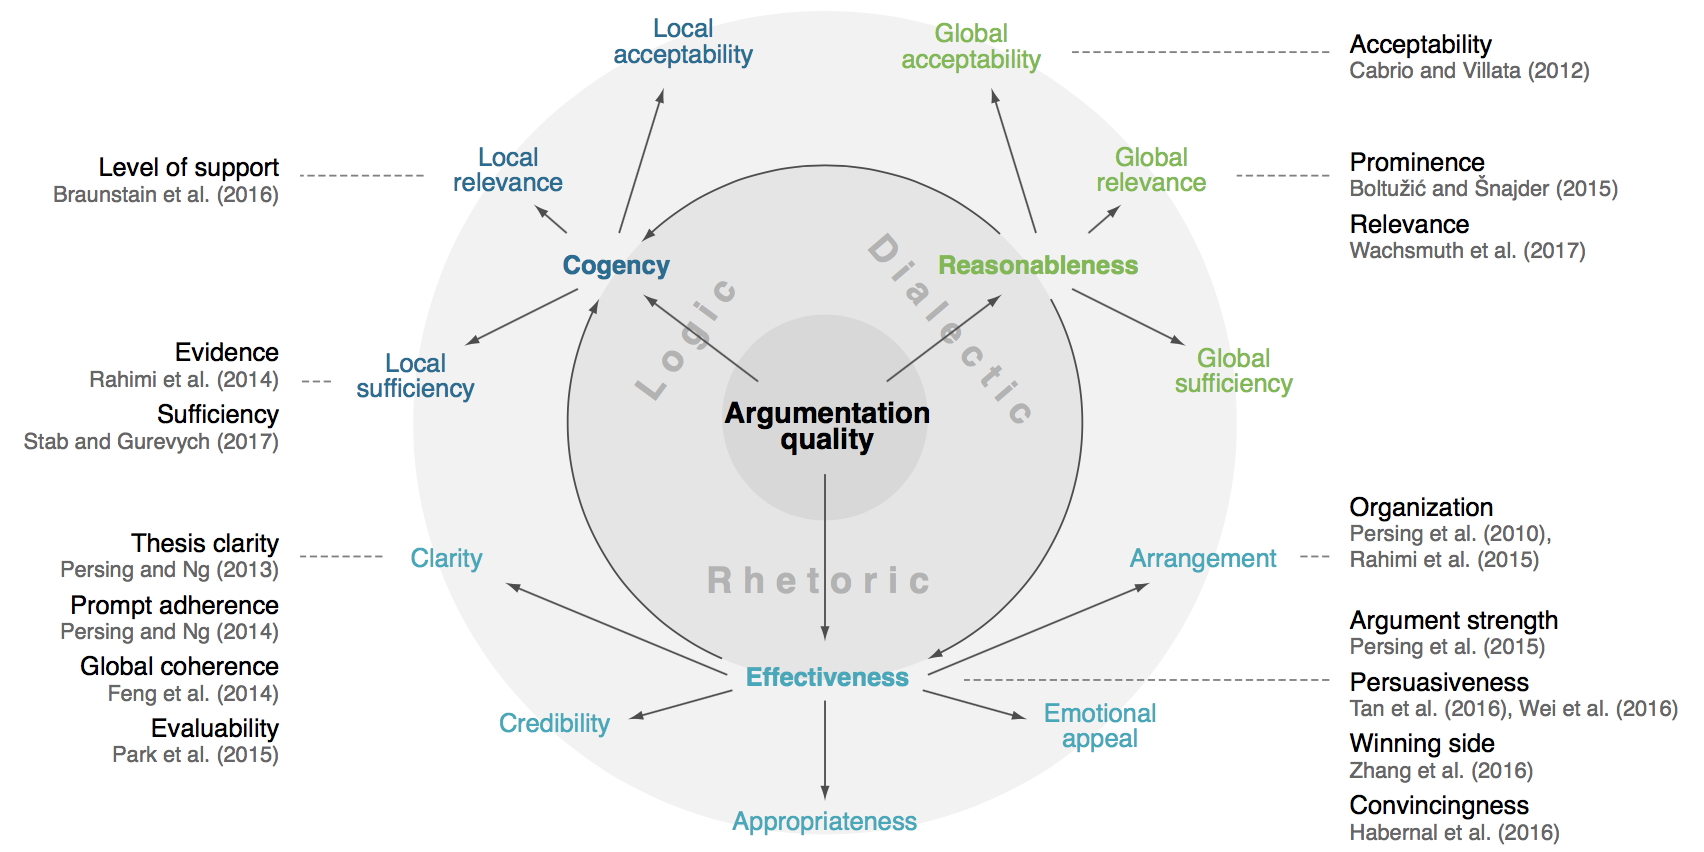
\includegraphics[width=\textwidth]{img/discussion-taxonomy}
			\caption{\small Wachsmuth, Henning, et al. ``Computational argumentation quality assessment in natural language.'' \textit{Proceedings of the 15th Conference of the European Chapter of the Association for Computational Linguistics: Volume 1, Long Papers}. Vol. 1. 2017.}
		\end{figure}
	\end{frame}
\end{document}
